\begin{frame}
\frametitle{Curse of dimensionality}
\begin{center}
{\Huge Large $p$, small $n$.\par}
\end{center}
\end{frame}

\begin{frame}
\frametitle{Nearest-neighbour classification}
\begin{columns}[c]
\column{0.7\textwidth}
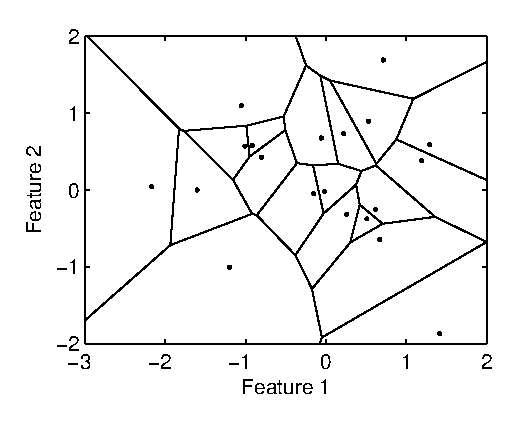
\includegraphics[width=\textwidth]{voronoi}
\column{0.3\textwidth}
\begin{itemize}
\item Not nice smooth separations.
\item Lots of sharp corners.
\item May be improved with \emph{K-nearest neighbours}.
\end{itemize}
\end{columns}
\end{frame}

\begin{frame}
\frametitle{Rule-based approaches}
\begin{columns}[c]
\column{0.7\textwidth}
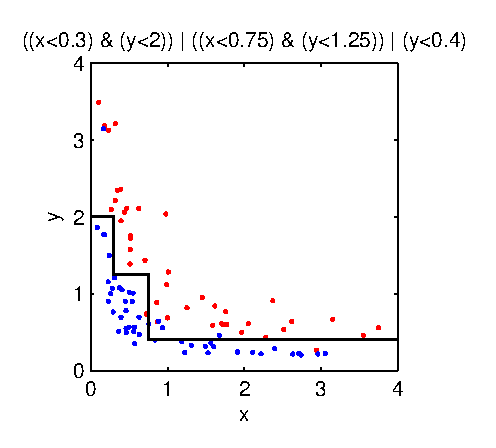
\includegraphics[width=\textwidth]{rule_based}
\column{0.3\textwidth}
\begin{itemize}
\item Not nice smooth separations.
\item Lots of sharp corners.
\end{itemize}
\end{columns}
\end{frame}


\begin{frame}
\frametitle{Corners matter in high-dimensions}
\begin{columns}[c]
\column{0.4\textwidth}
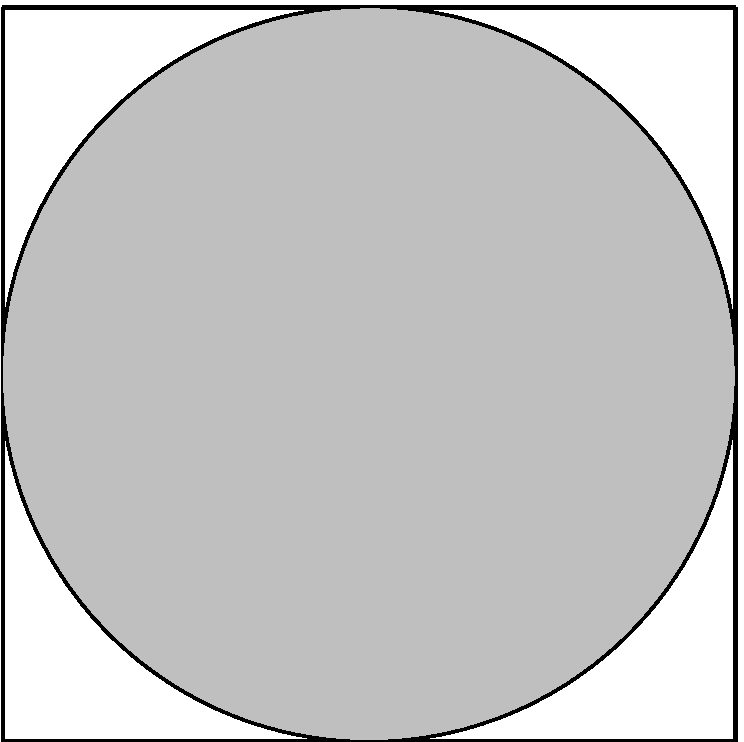
\includegraphics[width=\textwidth]{circle}
\column{0.6\textwidth}
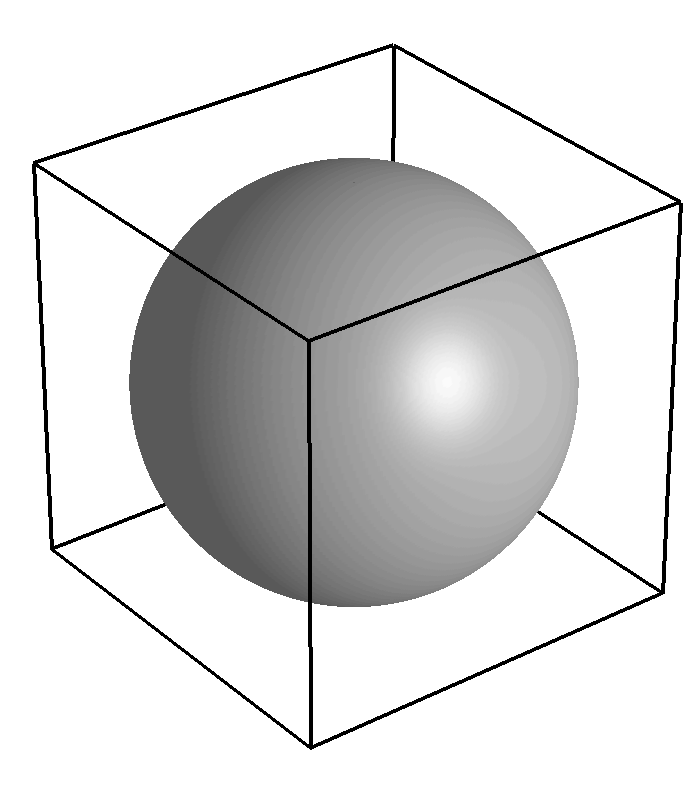
\includegraphics[width=\textwidth]{sphere}
\end{columns}
\end{frame}

\begin{frame}
\frametitle{Corners matter in high-dimensions}
\begin{columns}[c]
\column{0.2\textwidth}
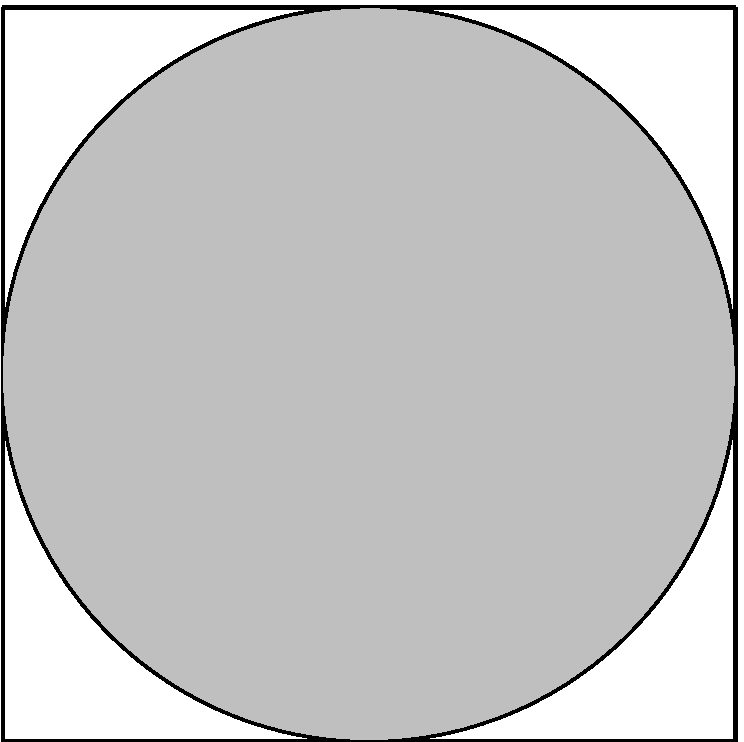
\includegraphics[width=.8\textwidth]{circle}

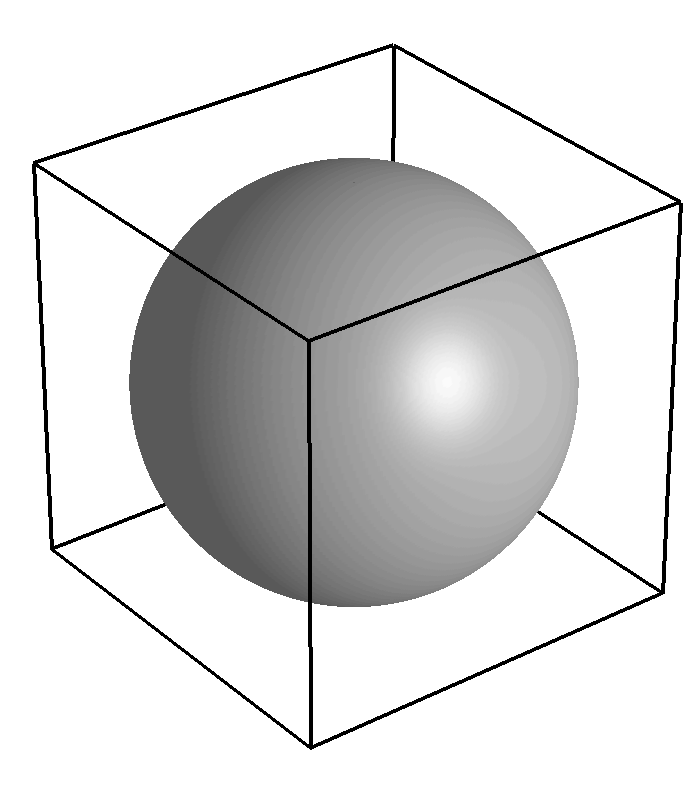
\includegraphics[width=\textwidth]{sphere}
\column{0.8\textwidth}
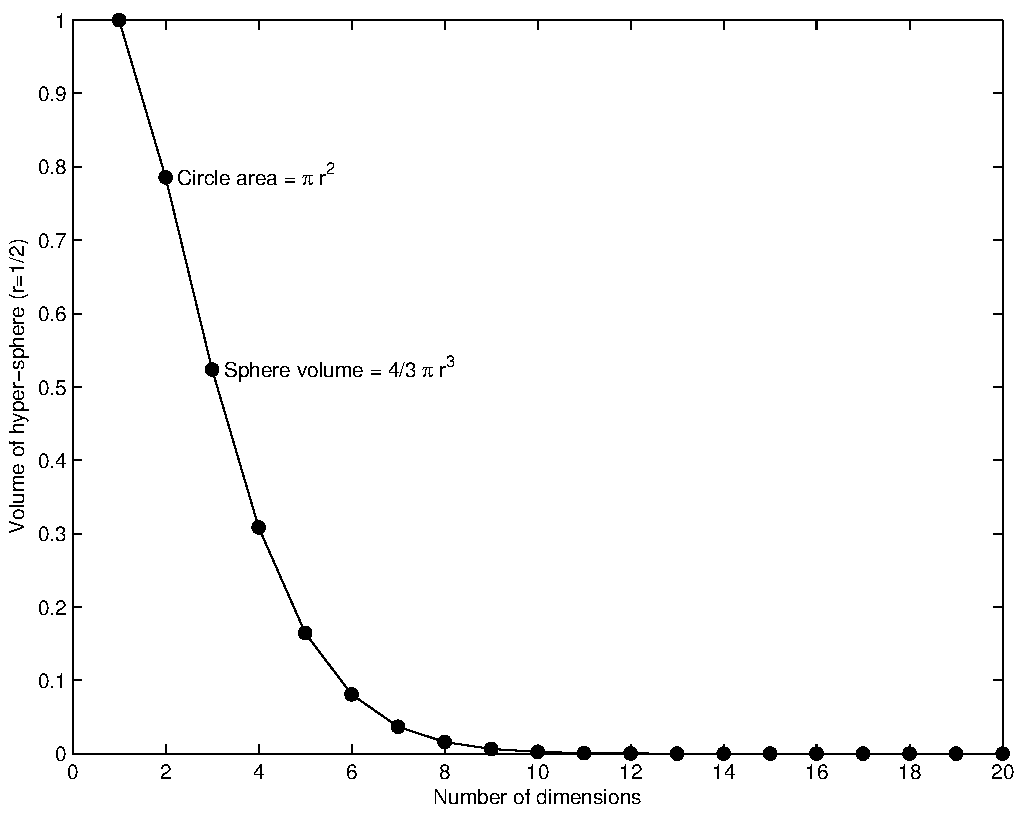
\includegraphics[width=\textwidth]{corners}
\end{columns}
\end{frame}

\begin{frame}
\frametitle{Dimensionality $\ne$ number of voxels}
\begin{itemize}
\item Little evidence to suggest that most voxel-based feature selection methods help.
\begin{itemize}
\item Little or no increase in predictive accuracy.
\item Commonly perceived as being more ``interpretable''.
\end{itemize}
\item Prior knowledge derived from independent data is the most reliable way to improve accuracy.
\begin{itemize}
\item e.g. search the literature for clues about which regions to weight more heavily.
\end{itemize}
\end{itemize}

\vspace{1cm}
{\tiny Cuingnet, R\'emi, Emilie Gerardin, J\'er\^ome Tessieras, Guillaume Auzias, St\'ephane Leh\'ericy, Marie-Odile Habert, Marie Chupin, Habib Benali, and Olivier Colliot. ``Automatic classification of patients with Alzheimer's disease from structural MRI: a comparison of ten methods using the ADNI database.'' Neuroimage 56, no. 2 (2011): 766-781.\par}
{\tiny Chu, Carlton, Ai-Ling Hsu, Kun-Hsien Chou, Peter Bandettini, and ChingPo Lin. ``Does feature selection improve classification accuracy? Impact of sample size and feature selection on classification using anatomical magnetic resonance images.'' Neuroimage 60, no. 1 (2012): 59-70.\par}
{\tiny See winning strategies in \url{http://www.ebc.pitt.edu/PBAIC.html}\par}
\end{frame}

\begin{frame}
\frametitle{Linear versus Nonlinear methods}
\begin{columns}[c]
\column{0.7\textwidth}
\begin{itemize}
\item Linear methods are more interpretable.
\item Nonlinear methods usually increase dimensionality.
\item Better to preprocess to obtain features that behave more linearly.
\end{itemize}
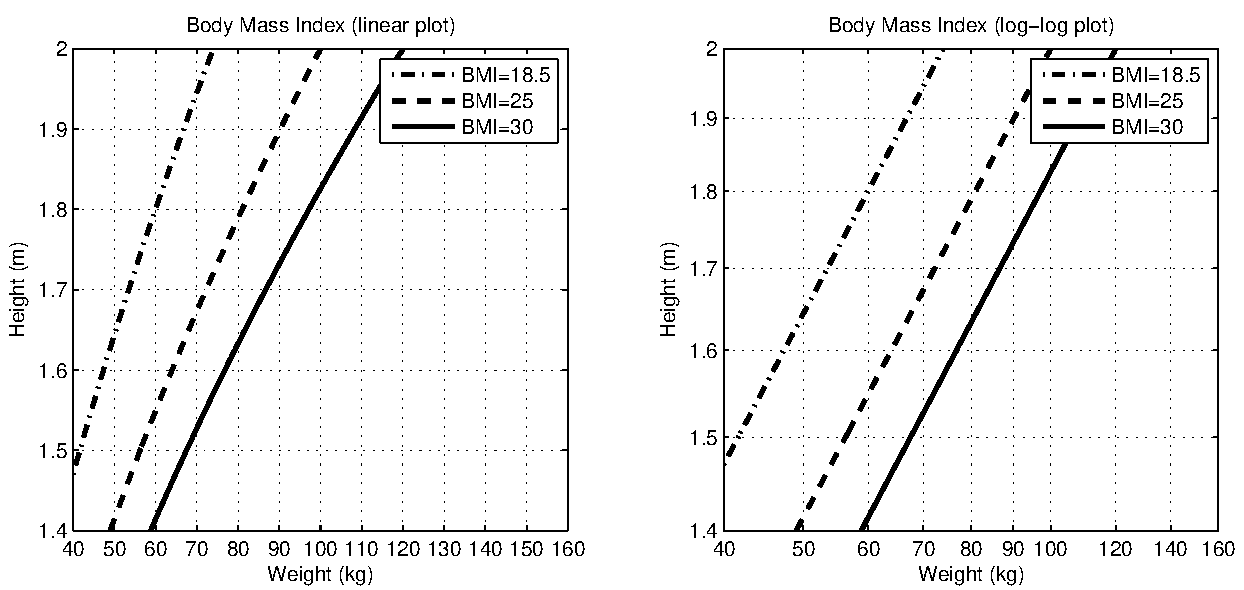
\includegraphics[width=\textwidth]{bmi}
\column{0.3\textwidth}
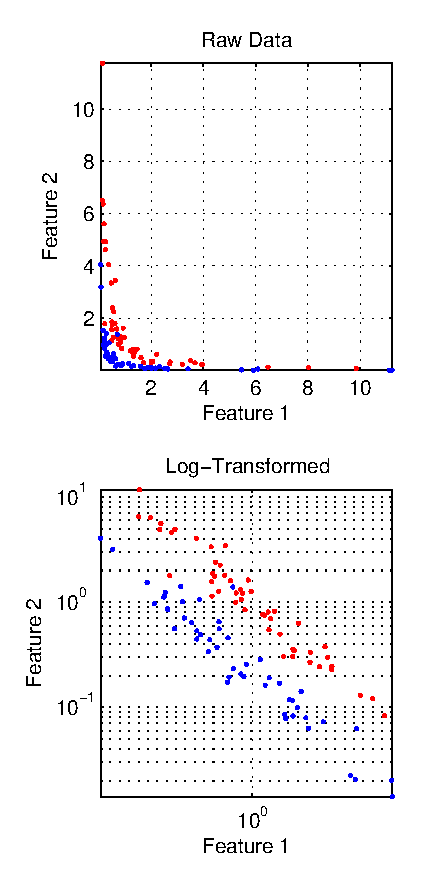
\includegraphics[width=\textwidth]{log_transformed}
\end{columns}
\end{frame}

